\subsection{Use Cases}
For at sikre at vi laver et program, der fungerer som ønsket, har vi opstillet flere use cases for systemet.
Disse use cases er blevet udledt på baggrund af møder med Psykolog Nords ledelse, og ved brug af de fire basis funktioner for persistens: create, read, update og delete (CRUD), på objekt- og domænemodelen. 
Det er f.eks. vigtigt at skelne mellem at booke en ny aftale, ændre den og aflyse den, da det er tre forskellige funktionaliteter i systemet.

\begin{figure}[p]
	\centering
  		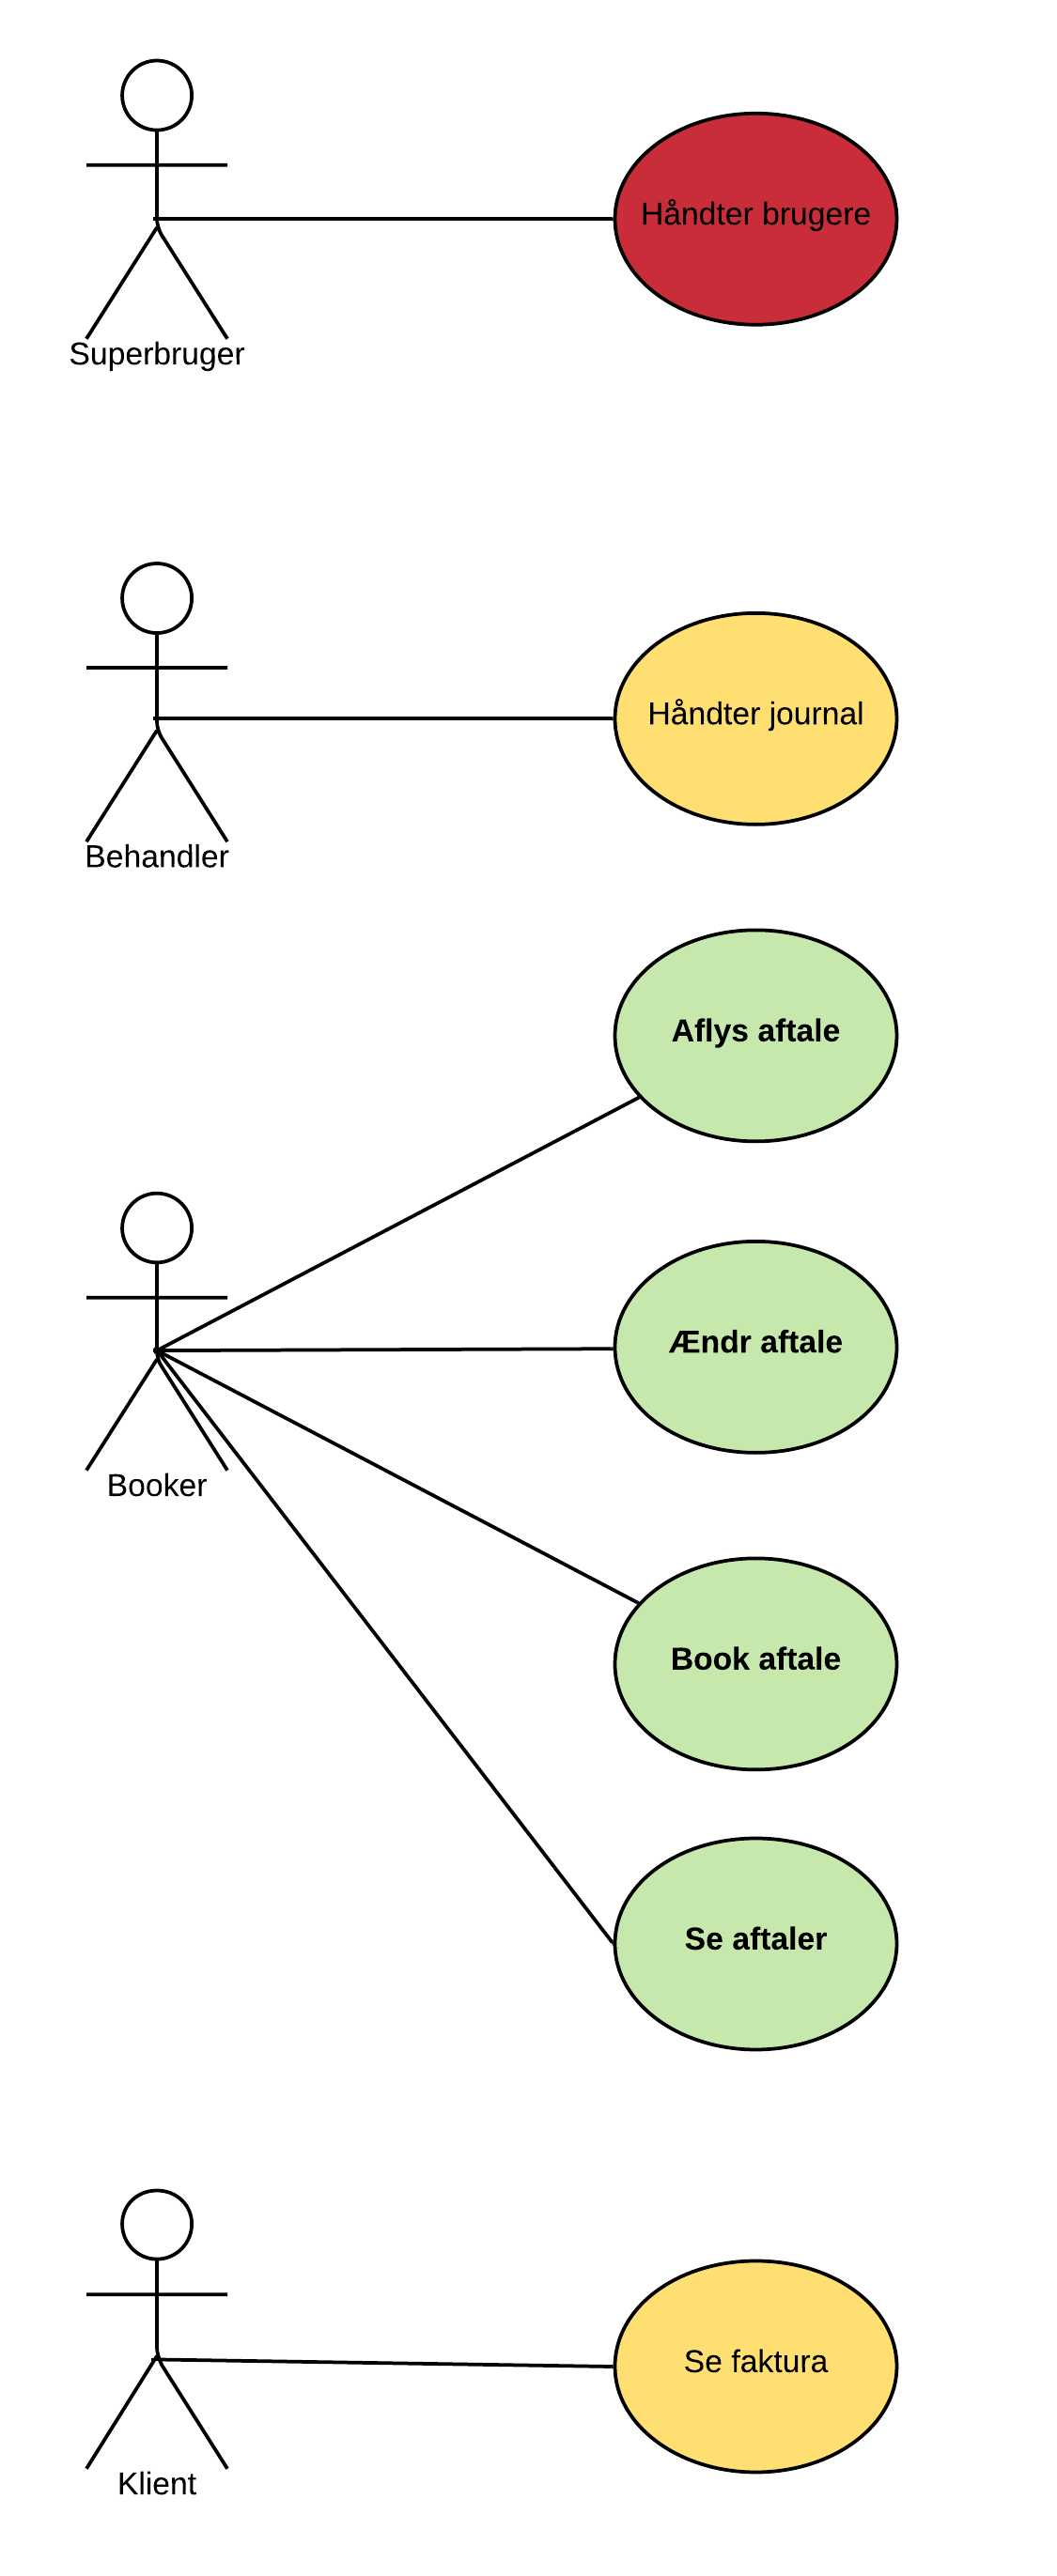
\includegraphics[scale=0.75]{UseCaseDiagram.png}
  \caption{Use Case diagram.}
  \label{fig:UseCaseDiagram}
\end{figure}

På figur \ref{fig:UseCaseDiagram} kan man se alle de use cases vi fandt frem til. 
I følgende kapitel kan man så findes vores use cases beskrevet mere detaljeret.

En aftale består af to aftaleparter: en klient og en bruger. 
Når der i dette afsnit bliver refereret til en aftalepart vil det være en af disse. 
Vi skelner ikke mellem hvilken af de to aktører, der er aftaleparten i de nedenstående use cases, da use casesene skal gælde for begge aktører.

\subsubsection{Use Case: Book aftale}\label{usecase:bookaftale}
{\setlength{\parindent}{0cm}
\textbf{Scope:} Bookingsystem for Psykolog Nord

\textbf{Primær Aktør:} Aftalepart

\textbf{Preconditions:} En aftale skal ikke eksistere på det givne tidspunkt for begge aftaleparter.

\textbf{Hovedscenarie (succes):} Booking af ny aftale.

Aftaleparten ønsker at booke en aftale. 
Han vælger at oprette en ny aftale, hvor den anden aftalepart har tid. 
Aftalen oprettes og psykologen notificeres.

\textbf{Alternativt scenarie:} Booking af ny aftale over telefon.

Aftaleparten ønsker at booke en aftale. Han ringer til den anden aftalepart og beder om en tid. Aftalen oprettes som i hovedscenariet.
}

\subsubsection{Use Case: Ændr Aftale}
{\setlength{\parindent}{0cm}
\textbf{Scope:} Bookingsystem for Psykolog Nord

\textbf{Primær Aktør:} Aftalepart 

\textbf{Preconditions:} En aftale eksisterer, og der er mere end 24 timer til aftalen.

\textbf{Hovedscenarie (succes):} Ændring af aftale.

Den første aftalepart går ind i systemet og ændrer aftalen til andet tidspunkt.
Den anden part modtager en notifikation med ændringen.

\textbf{Alternativt scenarie:} Ændring af aftale over telefon.

Klienten ringer til den anden aftalepart og beder om at få ændret aftalen. Aftalen ændres som i hovedscenariet.
}

\subsubsection{Use case: Aflys Aftale}
{\setlength{\parindent}{0cm}
\textbf{Scope:} Bookingsystem for Psykolog Nord

\textbf{Primær Aktør:} Aftalepart

\textbf{Preconditions:} En aftale eksisterer.

\textbf{Hovedscenarie (success):} Aflysning af aftale.

Aftaleparten går ind i system og aflyser aftalen.
Den anden part modtager notifikation om aflysningen og fakturaen slettes.

\textbf{Alternativt scenarie:} Aflysning af aftale over telefon.

Klienten ringer til den anden aftalepart og beder aftalen aflyst.
Aftalen aflyses som i hovedscenariet.

\textbf{Alternativt scenarie:} Aflysning af aftale inden for 24 timer af aftalens tid.

Klienten går ind i system og aflyser aftalen.
Den anden part modtager notifikation om aflysningen, men fakturaen sendes stadig til klienten.

\textbf{Alternativt scenarie:} Aflysning af aftale inden for 24 timer af aftalens tid over telefon.

Klienten ringer den anden aftalepart for at aflyse aftalen. Aftalen aflyses som i ovenstående scenarie.
}

\subsubsection{Use Case: Se faktura}
{\setlength{\parindent}{0cm}
\textbf{Scope:} Bookingsystem for Psykolog Nord

\textbf{Primær Aktør:} Klient

\textbf{Precondition: }faktura eksisterer

\textbf{Hovedscenarie (success):} Se faktura

Klienten går ind i systemet og finder listen over fakturaer. 
Han finder den ønskede faktura og får den vist.
}


\subsubsection{Use Case: Betal faktura}
{\setlength{\parindent}{0cm}
\textbf{Scope:} Bookingsystem for Psykolog Nord

\textbf{Primær Aktør:} Klient

\textbf{Precondition:} Faktura eksisterer.

\textbf{Hovedscenarie (success):} Betal Faktura

Som i Use Case: Se faktura, finder klienten fakturaen. Klienten betaler for fakturaen og modtager kvittering.
}